\documentclass[11pt]{book}
\usepackage{amsmath}
\usepackage{geometry}               
\usepackage{epstopdf}
\usepackage{hyperref}

\usepackage{amssymb}
\usepackage{graphicx}
\usepackage{braket}
\usepackage{paralist}
\usepackage{eufrak}
\usepackage{amscd}



\title{Notes}
\author{Zhu Yong Ting}
\def\bE{{\mathbb{E}}}
\def\bR{{\mathbb{R}}}

\def\eqlaw{{\stackrel{\text{(law)}}{=}}}
\def\tS{{\widetilde{S}}}
\def\tB{{\widetilde{B}}}
\def\tmu{{\widetilde{\mu}}}
\def\tsigma{{\widetilde{\sigma}}}
\def\abs#1{{\left|#1\right|}}
\def\E{{\mathrm{E}\,}}
\def\EE#1{{{\mathrm{E}}\left(#1\right)}}


\def\tX{{\widetilde{X}}}
\def\tM{{\widetilde{M}}}
\def\tx{{\widetilde{x}}}
\def\tm{{\widetilde{m}}}

\begin{document}
\maketitle
\chapter{introduction}
\section{option}

An {\it option} is a contract which gives the holder the right but not the obligation to buy or sell an underlying asset by a certain date at an agreed price, as mentioned in \cite{Hull2008}.
To get this right, the buyer should pay the seller. The price set in the contract is known as the {\it strike price}; the date is known as {\it expiration date} or {\it maturity}. There are always two sides involved in every option contract. On one side is the investor who has bought the option. This side is known as the long position. Another side is the short position who has sold the option. A {\it call} option gives the holder the right to buy the underlying asset, while a {\it put} option gives the holder the right to sell the underlying asset. European options can be exercised only at the expiration date. American options on the other hand may be exercised at any time before the expiration date. 
% add more Brodie option pricing: valuation models and applications and the market share from Value at risk

Usually, there are five factors affecting the price of a stock option:
\begin{enumerate}[1.]
\item The current stock price, $S_0$
\item The strike price, $K$
\item The time to maturity, $T$
\item The volatility of the stock price, $\sigma$
\item The risk-free interest rate, $r$
\end{enumerate}

For European option, the payoff from a long position is $(S_T - K)^+$. As for American option, the payoff function is similar, what is different is we should use the stock price when the option is executed to calculate payoff, instead of $S_T$ in European case. 



Usually there are closed form price formulas for European options. In addition numerical approaches can solve this problem, such as binomial tree and Monte Carlo simulation. We will give a brief introduction about these numerical methods later. Because we do not know when American option will be excised, the pricing of American option is more complicated. A complete solution to American option pricing problem should address two aspects, option value and an optimal exercise strategy. Only in a few cases are analytic solutions available. In most cases, numerical approach is needed. Lim and Lai \cite{Lim2004} propose an approach to compute both the price and the optimal exercise boundary. 



\section{Black-Scholes model}   
The most popular model to describe stock price behavior is known as Black-Scholes model. Let $S_t$ be the stock price. Then under this model, $S_t$ satisfies this equation: 
\begin{equation}\label{eq:1}
dS_t = \mu S_tdt + \sigma S_tdB_t, 
\end{equation}
with $\mu$ and $\sigma $ constant, $B$ a standard Brownian motion. This approach to model stock price was first introduced by Black, Scholes and Merton. Denote $r$ as the constant continuously compounded risk-free interest rate. Under risk-neutral assumption, we can get $\mu = r $. 

If we define $G = \ln S$, after some calculation, we get 
\begin{equation}\label{eq:2}
dG_t = \frac{\mu - \sigma ^2 }{2} dt + \sigma dB_t.
\end{equation}
From this we can see that the natural logarithm of stock price is Brownian motion with drift $\mu$, and variance $\sigma^2$. This model implies that the stock's price at a given time $T$ follows lognormal distribution. The standard deviation of the logarithm of the stock price is $\sigma \sqrt{T}$. 

Black et. al. \cite{Black:1973} pointed out that the proper price of an option should be the expected present value of its payoff. Based on this idea, there are many studies about the pricing of options. For European plain vanilla option, its price can be priced in closed form. As for American plain vanilla option, because it can be executed at any time before maturity, the pricing is much more complicated. In this case, it is a optimal stopping problem. Comparing to vanilla option, there are another school of options called exotic options. Exotic options are nonstandard options created by financial engineers, which usually only traded in over-the-counter market. Although exotic options are a relatively small part of financial market in terms of volume, these options are important to investment banks because they are generally much more profitable than plain vanilla option. Usually, these options are path dependent. One typical exotic option is lookback option.

%In the this case, one can deduce that the optimal stopping time is given by some region. Precisely, the holder excise the option when stock price enter some region. 

% add something about path dependent option, particularly Asian option. 

\section{Lookback options}
Lookback options give the hold the right to capture the difference between asset price when the option is executed and maximum or minimum asset price reached during the life of the option. For a European style lookback call option, the payoff is the amount that the final asset price exceeds the minimum asset price attained during the life of the option. As for the put option, the payoff is the amount by which the maximum asset price attained during the life of the option exceeds the final asset price. Goldman etl firstly provided the valuation formulas for European lookbacks. In Hull \cite{Hull2008}, the value of a this type call option is 
\begin{equation}\label{eq:3}
S_0e^{-qt}N(a_1) - S_0 e^{-qT}\frac{\sigma ^2}{2(r-q)} N(-a_1) - S_{\min} e^{-rT}(N(a_2) - \frac{\sigma^2}{2(r-q)} e ^{Y_1} N(-a_3) 
\end{equation}
where
\begin{equation}\label{eq:4}
\begin{split}
a_1 &=\frac{\ln(S_0 / S_{\min}) + (r-q+\sigma^2 /2)T}{\sigma \sqrt{T}}\\
a_2 &= a_1 - \sigma \sqrt{T}\\
a_3 &= \frac{ln(S_0 / S_{\min})+ (-r+q+\sigma^2 / 2)T}{\sigma \sqrt{T}}\\
Y_1 &= - \frac{2(r-q-\sigma^2 / 2) \ln(S_0 / S_{min})}{\sigma^2}
\end{split}
\end{equation}
and $S_{\min}$ is the minimum asset price achieved to date. 
The value of a European lookback put is 
\begin{equation}\label{eq:5}
S_{\max} e^{-rT} ( N(b_1) - \frac{\sigma^2}{2(r-q)} e^{Y_2} N(-b_3)) + S_0 e^{-qT}\frac{\sigma^2}{2(r-q)} N(-b_2) - S_0 e^{-qT} N(b_2)
\end{equation}
where 
\begin{equation}\label{eq:6}
\begin{split}
b_1 &= \frac{\ln(S_{\max} / S_0) + (-r + q + \sigma^2 /2)T}{\sigma \sqrt{T}}\\
b_2 &= b_1 - \sigma \sqrt{T}\\
b_3 &= \frac{\ln(S_{\max} / S_0) + (r-q-\sigma^2 /2)T}{\sigma \sqrt{T}}\\
Y_2 &= \frac{2(r-q-\sigma^2 / 2) \ln(S_max / S_0)}{\sigma^2}
\end{split}
\end{equation}
and $S_{\max}$ is the maximum asset price achieved to date. 

These formula are got under the assumption that the asset price is observed continuously. However, in real life, the asset price is observed discretely. Broadie etl. \cite{Broadie1999} give a creation to these formulas to deal with discrete situation. For the discrete options, let $m$ be the number of price-fixing dates and $\Delta = T/m$ the interval between fixing. In their paper, we can find that the price of a discrete lookback at the $k-th$ fixing data and the price of a continuous lookback at time $t = k \delta t$ satisfy
\begin{equation}\label{eq:7}
V_m (S_\pm) 
= 
e^{\mp\beta_1 \sigma \sqrt{\frac{T}{m}}} 
V(S_{\pm}e^{\mp\beta _1 \sigma \sqrt{\frac{T}{m}}} + 
(e^{\mp \beta_1 \sigma \sqrt{\frac{T}{m}}} -1)S_t + o(1/\sqrt{m})
\end{equation}
where, in $\pm$ and $\mp$, the top case applies for puts and the bottom for calls, and $\beta_1 = \lim_{m\to\infty} \frac{\sqrt{m}E[\max_{0\leq t \leq T} B_t - \max_{0\leq k \leq m} B_{kT/m}]}{\sigma \sqrt{T}}$. 

By this correction,we can use continuous pricing formula
to value discrete loolback. To get a more precise value for put,
first we should inflate the predetermined max by a factor of
$e^{\beta_1 \sigma \sqrt{T/m}}$,
then deflate the expected maximum over $[0,T]$ by the same factor. For a lookback call, first deflate the predetermined min, then inflate the expected minimum. 

As for American option, the complete solution should provide both the option value and an optimal exercise strategy. Due to this complicity, usually we need use numerical approach to solve the problem of pricing American style lookback option. In Lim and Lai \cite{Lim2004}, for American $fixed$ $strike$ lookback option they provide an full approach to compute the price and the optimal exercise boundary. In this paper, they first propose a space-time transformation which can reduce the valuation of a group of American lookback options to a single canonical optimal stopping problem for standard Brownian motion. Under this transformation, calendar time is scaled by the by square of volatility. Therefore, the canonical time horizon is only a small part of time to expiration. In addition, the transformation also removes the dependence on a prescribed root node which then make computing the entire early excise boundary by backward induction possible.  

%Fix a process $X_t$, define $M_t = \max_{0\leq s\leq t} X_s$. 
%When $X_t$ is a standard brownian motion without drift, 
%the joint distribution of $M_t$ and $X_t$ can be easly calculated by reflection principle\cite{Karatzas91}:
%\[ 
%P(X_t \in a+dx, M_t \in b+dm) =  
%\]


\section{$\alpha$-quantile}
For a stochastic prcess $X_t$,
the $\alpha$-quantile $( 0 \leq \alpha \leq 1)$ 
is defined by 
\[
M(\alpha,t)(\omega) = \inf\Set{x:\int_0^t 1_{(X_s (\omega)\leq x)} > \alpha t}.
\]
Then we can see that $\inf_{0\leq s \leq t}  X_s = lim_{\alpha\to 0}M(\alpha,t)$ and $\sup_{(0\leq s \leq t})  X_s = lim_{\alpha\to 1} M(\alpha, t)$. In this sense $\alpha$-percentile option can be considered as a general class of lookback option. Unlike lookback option whose payoff depends on the maximum or minimum of the price of sock before maturity as mentioned before, $\alpha$-percentile option's payoff depends on the quantile of the stock price process. This option was first introduced by Miura\cite{Miura} in 1992. In 1995, Akahori\cite{Akahori1995} gave a generalized arc-sine law for this type of options by Feynman-Kac formula.
When $X_{t}$ is a Brownian motion $B_t$, using similar mathematical tools, Dassios obtained the explicit density of quantile option and gave a exceptional representation of the distribution of quantile.  In \cite{Dassios1995}, for $\alpha\in[0,1]$, $t\leq 0$, Dassios proved that 
\begin{equation}\label{eq:Dassios}
M(\alpha, t) \eqlaw \sup_{s \leq \alpha t} X_s + \inf_{s\leq (1-\alpha)t} X'_s ,
\end{equation}
where $X'$ is a independent copy of $X$. Later in 1995, Embrechts, Rogers and Yor \cite{EmRoge1995} gave two proofs of this theorem without using Feynman-Kac computations. 
\subsection{The advantage of $\alpha$-quantile option}
\cite{Ballotta}
\subsection{The distribution function of $\alpha$-quantile of Brownian motion}
In 1995, Yor gave the distribution function of the $\alpha$-quantile of Brownian motion without drift in \cite{Yor1995}. He obtained this result by simplifying related integral expressions on Miura \cite{Miura}. When $\mu = 0$, that is Brownian motion $B_t$ is without drift, define $\theta = ((1 - \alpha)/(\alpha))^{1/2}$, for the Brownian quantiles on time interval $[0, 1]$,  in \cite{Yor1995} we find:
\begin{equation}
P(M(\alpha,1)\in dx)= \begin{cases} 
\sqrt{2 / \pi}exp(-x^2 / 2) \Phi(|x| / \theta)dx  &  \text{if } x \leq 0 \\
\sqrt{2 / \pi}exp(-x^2 / 2) \Phi(\theta x)dx  &  \text{if } x \geq 0 
\end{cases}
\end{equation}
where 
\begin{equation}\label{eq:density}
\Phi (x) = \sqrt{2/ \pi} \int^{\infty}_x dy exp(-y^2 / 2) = P (|N| \geq x)     (x \geq 0),
\end{equation}
with $N$ a standard Normal random variable. 


When $u \neq 0$, Dassios  in \cite{Dassios1995} addressed this question for a more general case.  As stated in equation (\ref{eq:Dassios}), the density of 


\subsection{Tree method for European Option}
Like lookback option, quantile option is also path-dependent. What makes things difficult is that quantile option is not markov. Normal tree methods which usually involve backward induction do not work in this case. We need to record all the information of the path because of lack of markov property, which will lead the tree to explosion computationally. 
Kwok and Lau in \cite{Kwok2001} proposed a special way to apply tree method to price quantile option. In this paper, they find a relation between the price of quantile option and the price of cumulative Parisian option. By this approximation, they can simplify the pricing of quantile option. In their paper, they assume that there are $M$ time steps for the whole monitoring period $[0,T]$, and they define ${S^M}_j$, $j = - M$, ...$0$,$1$,...,$M$ as the discrete asset prices at maturity. Under trinomial tree method, the possible prices happened in one tree are limited to ${S^M}_j$,  $j = - M$, ...$0$,$1$, ...,$M$, which is also true for the value taken by quantile of brownian motion. Therefore they derived that 
\begin{equation}\label{eq:kowk1}
V(\alpha, T) = e^{-rT} \sum^{M}_{j=-M}P[M(\alpha,T)=S^{M}_{j}]\max(S^{M}_{j}-X,0),
\end{equation}
where $V(\alpha,T)$ is for the value of $\alpha$-quantile option whose maturity it $T$, $P[M(\alpha,T)=S^{M}_{j}]$ is the probability that the quantile of Brownian motion achieve the value ${S^M}_j$,  $j = - M$, ...$0$,$1$, ...,$M$. In their paper, they observed that the difference between the prices of two cumulative Parisian binary options is a good approximation for $P[M(\alpha,T)=S^{M}_{j}]$ multiplies discount factor $e^{-rT}$, ie.
\begin{equation}\label{eq:kowk2}
e^{-rT}P[M(\alpha,T)=S^{M}_{j}] \approx V^{bin}_{cum}[(1-\alpha)T, S^{M}_{j-1}]-V_{cum}^{bin}[(1-\alpha)T, S_{j}^{M}]  
\text{ for }j=-M, ... , 0, 1, ... , M
\end{equation}
where $V^{bin}_{cum}[d,B]$ is denoted as the price of continuously monitored cumulative Parisian binary option with down barrier $B$, and $d$ be the minimum cumulative time staying above the down barrier to avoid knock-out. 


Combining equation (\ref{eq:kowk1})and (\ref{eq:kowk2}), they get
\begin{equation}\label{eq:kowk3}
V_{alp} = \sum^M_{j=-M} \max (S^M_j - X,0) \times \{V_{cum}^{bin}[(1-\alpha)T, S^M_{j-1}] - V^{bin}_{cum}[(1-\alpha)T, S^M_j]\} ,
\end{equation}
where $V^{bin}_{cum}[(1-\alpha)T, S_{-(M+1)}^M] = e^{-rT}$. By this result, we can turn pricing of quantile option into pricing of $2M+1$ cumulative Parisian option. 


Parisian option is like an advanced version of barrier option. We know barrier option are options where the payoff depends on whether the underlying asset's price reaches a certain level (barrier) during the option's life. Barrier options usually trade in the over-the counter market. This kind of option is attractive because it is usually cheaper than similar option without barrier. Like vanilla option, barrier options also authorize holders the right to buy or sell, but  long sides of barrier options do not need to pay for scenarios they think is unlikely to happen in the future. One good example I find from wikipedia is about IBM. If you believe that IBM will go up this year, but are willing to bet that it won't go above \$100, then you can buy the barrier and pay less premium than the vanilla option. But in this one-touch knock-out or knock can bring difficulties to option writers when asset price is close to barrier. Particularly in the foreign exchange market where manipulation of underlying asset price is not impossible. To overcome short period price manipulation, various adjustments to one-touch knock out or knock in have been performed in practice. Parisian option is one solution.  In order to get activated, the underlying assets of parisian option need to stay in the knout out or knout in region for certain period of time. The payoff of a cumulative Parisian option is dependent on the total amount of time the underlying asset price has spent above or below barrier. As for binary option, the payoff is either some fixed amount of some asset or nothing at all. 

\subsection{pricing cumulative parisian binary option by FSG}
Kwok and Lau also proposed a forward shorting grid(FSG) to price cumulative parisian option in \cite{Kwok2001}. The character of FSG is that this approach need add additional information at each node of  a lattice tree. Commonly in pricing path-dependent option, at each node we should add state vector to represent the path-dependent attribute, such as the extreme value of the underlying asset price achieved in lookback option case. As we know Hull and White \cite{Hull1993} and Ritchken, Sankarasubramanian and Vijh \cite{Vijh1993} were the first authors suggested this approach. In 1996, Barraquand and Pudet \cite{Barraquand1996} introduced a comprehensive framework for FSG. In this paper they indicated that the FSG method is unconditionally convergent. Further, they showed that when the covariance matrix is degenerate, the FSG method can outperform finite difference methods. The convergence of the FSG algorithm in pricing of Asian options was studied by Forsyth, Verzal and Zvan \cite{Forsyth1999}. Foesyth et al. pointed out that    
 
 In Kwok and Lau's paper\cite{Kwok2001}, they constructed a trinomial tree to get the price of cumulative parisian option. But due to the fact that the result is not steady according to the setting of the length of up movement between each immediate steps, we modify their method to binomial tree. 
 
In building binomial tree, we start by cutting the entire life of one option into many small time intervals of length $\Delta t = T / M$. 
Our tree is build to mimic the the logarithm process of underlying asset price. Denote $x=\ln S$. In each step, the logarithm of the price of underlying asset is assumed to move from its initial value of $x_0$ to one of the two new values, $x_0 + d + u$ and $x_0 + d - u$ with equal probability,that is $p_{up} = p_{down} = 0.5$ , where $u = \sigma \sqrt{\Delta t}$ and $d = (r - {\sigma}^2 /2)\Delta t$. Here $\sigma$, and $r$ are volatility and riskless interest rate, respectively. The model is illustrated in Figure~\ref{fig:tree1}.  
\begin{figure}[htbp]
   \centering
   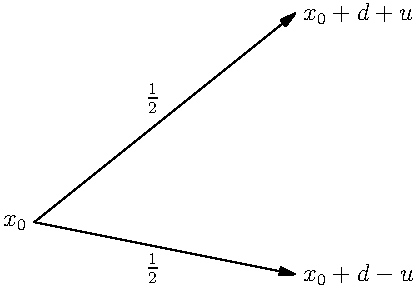
\includegraphics{trees.pdf} % requires the graphicx package
   \caption{Forward shooting}
   \label{fig:tree1}
\end{figure}

Like the notation used in \cite{Kwok2001}, we denote $V[m,j;k]$ as the numerical option value of the cumulative parisian option at the $m$-th time interval,  $j$ upward jumps from the initial underlying asset value and $k$ times breaches so far. Let $g(k,j)$ be the grid function that describes the correlated evolution of number of breaches $k$ and price indicate $j$. Denote $x_j$ be the value of $x$ corresponding to $j$ upward movements on the binomial tree. Then we should add $1$ to the indicator $k$ if the underlying asset price $S$ is no more than the barrier $B$; i.e $x_j \leq \ln B$. Hence we can see that a suitable setting of the grid evolution function $g(k,j)$ should be 
\begin{equation}\label{eq:grid}
g(k,j) = k + 1_{\Set{x_j \leq B}}
\end{equation}
where $1_{\set{x_j \leq B}}$ is the indicator function. It is defined as 
\begin{equation}\label{eq:grid-indicator}
1_{\Set{x_j \leq B}} =  \begin{cases}
1 & \text{if } x_j \leq \ln B \\
0 & \text{if } x_j > \ln B
\end{cases}
\end{equation}
Then the FSG method for pricing the cumulative Parisian binary option can be expressed as
\begin{equation}\label{eq:fsg}
V[m-1,j;k] =\set{0.5V[m,j+1;g(k,j+1)]+0.5V[m,j-1,g(k,j-1)]}e^{-r\Delta t} 
\end{equation}
for $m-1 < M$. 


Let $N$ be the predetermined number of breaches recored for the all duration of the life of an option that is desired to activate   the contract. 
Considering the binary feature of the option, we should initiate our algorithm with
\begin{equation}\label{eq:initiate}
V[M,j;k] = \begin {cases}
1 & \text{if }  k < N \\
0 & \text{if }  k \geq N
\end{cases}
\end{equation}
By (\ref{eq:initiate})  (\ref{eq:fsg}) and backward induction, we can get the price of cumulative Parisian binary option with any prescribed times of breaches and barrier. 

Recall what we get by equation (\ref{eq:kowk2}). In order to get the price of $\alpha$-quantile option, we can use the prices of $2M + 1$ cumulative Parisian binary options to approximate $\alpha$-quantile option's value. Hence using the FSG method we described above to calculate the prices of cumulative Parisian option  and doing a simple math work by equation (\ref{eq:kowk2}), we can get the approximated price for $\alpha$-quantile option with $M$ time steps.  

Recall we defined earlier $\Delta t = T / M$. We compute the approximated option price of an $\alpha$-quantile call option with different time steps using equation (\ref{eq:kowk2}). As you can see in Figure % add figure ,
the numerical values of option are plotted against varying $\Delta t$. The values of parameters of the $\alpha$-quantile call option are set as: $ \alpha = 0.8$, $S_0 = 100$, $X = 95$, $r = 5\%$, $\sigma = 20\%$, and $T = 0.25$. 
\begin{figure}[htbp]
   \centering
   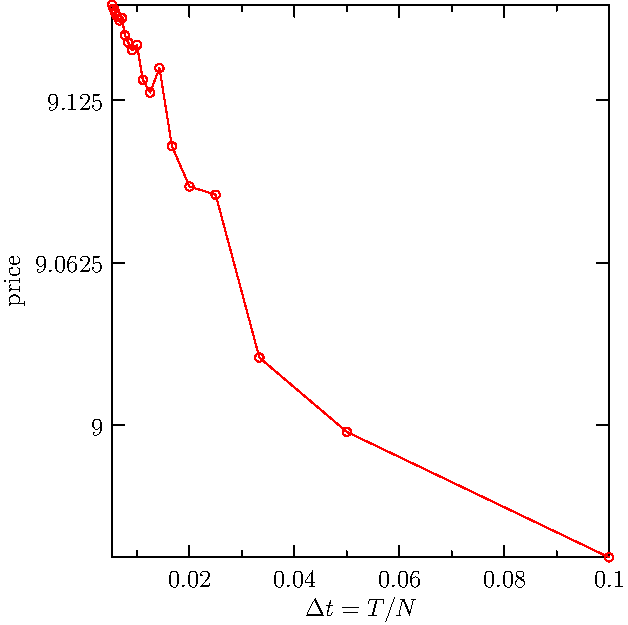
\includegraphics{bfsg.pdf} % requires the graphicx package
   \caption{example caption}
   \label{fig:2}
\end{figure}


\subsection{ an exponential time tree for American $\alpha$-quantile option}
% to be add
 
 











\section{Discrite v.s. continous}
\subsection{Euler scheme and randon walk}
approximate brownian by random walk through Euler scheme.


\subsection{path transform}
Let $S_k$ be a randon walk (assume $S_0=0$) 
with i.i.d increasment, i.e. 
$\Delta S_k = S_k -  S_{k-1}$ is i.i.d. 
Define the ordered statistics $M_{k,n}$ be the $k$th-smallest value in
$\Set{S_i}_{i=0}^n$. 
Under this setting, clearly, $M_{0,n} = \inf_{0\leq i\leq n}S_i$
and $M_{n,n} = \sup_{0\leq i\leq n}S_i$
Define 
\[S'_i = S_{i+k}-S_k\] 
for fixed $k, n$.  

In Wendel's paper\cite{Wendel1960}, an identity about randon walk with 
i.i.d increasment was dirived:
\begin{equation}\label{eq:dpathdec}
(M_{k,n}, S_n) \eqlaw (\sup_{i\leq k} S_i +\inf_{i\leq n-k} S'_i, S_n)
\end{equation}

In 
\cite{Chaumont1999}, Chaumont provide a combinatorics treatment. 
He constructed a explicit path transform for $S$ to $\tS$, such that 
\[
(M_{k,n}, S_n) = (\sup_{i\leq k} \tS_i+\inf_{i\leq n-k} \tS'_i, \tS_n)
\]
Here $\tS$ has same distribution with $S$ and each path $S$
 one-one corresponed to $\tS$.

By using path transform, Chaumont proved 
following continous version of path decomposition:
\begin{equation}\label{eq:cpathdec}
(M_{\alpha,T}, S_T) \eqlaw (\sup_{t\leq \alpha{T}} S_T +\inf_{t \leq (1-\alpha)T} S'_t, S_T)
\end{equation}
where as above:
\[
S'_t = S_{\alpha T+t} - S_{\alpha_T}.
\]

For Brownian motion case, this formular were proved in many differet ways
and original due to Dassios\cite{Dassios1995}. 

\subsection{an estimate of week discrete error}
\cite{Janssen2008} gives a estimate of the difference of  expatations 
between maximum of borwnian motion and associated random walk.  
Since we just give a really rough estimate, we only list the first two term. 
For $B_t$ a Borwnian motion with drift $\mu$ and variance $1$ on time interval $[0,1]$, that is $B_t = \mu t + W_t$, where $W_t$ is standard Brownian motion, we can get
\begin{equation}\label{eq:est1}
E\max_{0\leq t \leq 1} B(t) - E\max_{n=0,\cdots, N}B(n/N) 
= -\frac{\zeta(1/2)}{\sqrt{2\pi N}}-\frac{2g(1)-\mu}{4N} + O(1/N^{3/2})
\end{equation}
where 
\[
g(t) = \mu \Phi(\mu \sqrt{t}) + \frac{1}{\sqrt{2\pi t}} e^{-\frac{1}{2}\mu^2 t}.
\]
\[
\zeta(1/2) \approx -3.92264613.
\]

For general Borwnian $\tB(t)$ motion on time interval $[0,T]$ with drift $\tmu$, variance $\tsigma$, 
we use following transform
\begin{align*}
\tB_t &= \tsigma \sqrt{T} B_{t/T} = \tsigma \sqrt{T} \mu t/T 
+ \sqrt{T}\tsigma W_{t/T}\\
\mu &= \tmu \sqrt{T}/\tsigma 
\end{align*}
do derive the follwoing formula:
\begin{equation}\label{eq:maxest}
E\max_{0\leq t\leq T} \tB(t) - E \max_{0\leq n \leq N} \tB(nT/N) = 
 -\frac{\zeta(1/2)}{\sqrt{2\pi}}\tsigma \sqrt{T/N}
 -\frac{2g(1)-\tmu\sqrt{T} / \tsigma}{4N}\tsigma\sqrt{T} + 
O(\sqrt{T}/N^{3/2})
\end{equation}

Now combine $(\ref{eq:cpathdec})$ $(\ref{eq:dpathdec})$ and $(\ref{eq:maxest})$, for $0 < \alpha < 1$, 
we get an very rough estimate of the apporximation order:
\begin{equation}
\begin{split}
\E (M_{\alpha,T}) - \E (M_{k,N})
=& \EE{\sup_{t\leq \alpha{T}} S_t +\inf_{t \leq (1-\alpha)T}S'_t} 
- \EE{\sup_{i\leq k} S_i+\inf_{i\leq N-k} S'_i}\\
=& \EE{\sup_{t\leq \alpha{T}} S_t +\inf_{t \leq (1-\alpha)T}S'_t
-  \sup_{i\leq k} S_i-\inf_{i\leq N-k} S'_i} \\
= &  \EE{\sup_{t\leq \alpha{T}} S_t - \sup_{i\leq k} S_i} +
\EE{\inf_{t \leq (1-\alpha)T} S'_t-\inf_{i\leq N-k} S'_i}\\
=& -\frac{\zeta(1/2) \tsigma}{\sqrt{2\pi}}\left(\sqrt{T/\alpha N} 
\sqrt{\alpha} - \sqrt{T/(1-\alpha)N}\sqrt{1-\alpha}\right) \\
& - \frac{2g(1)}{4}\sqrt{T} \tsigma
\left(\frac{1}{\alpha N} \sqrt{\alpha} 
  - \frac{1}{(1-\alpha)N}\sqrt{1-\alpha}\right) \\
& + \tmu \left( \frac{1}{4\alpha N}\alpha
  +\frac{1}{4(1-\alpha)N}(1-\alpha)\right)T
+ O(\sqrt{T}/N^{\frac{3}{2}}) \\
=& - \frac{2g(1)\sqrt{T}\tsigma}{4N}
\left(\frac{1}{\sqrt{\alpha}} 
  - \frac{1}{\sqrt{1-\alpha}}\right) \\
& + \frac{\tmu T}{2 N}
+ O(1/N^{\frac{3}{2}}) 
\end{split}
\end{equation}
where $k = \alpha N$.
The second last equality holds by view $\inf_{t\leq (1-\alpha)T} S'_t$ as 
$-\max_{t\leq (1-\alpha)T} (-S'_t)$.

This estimate shows that the convergence order 
are all $\frac{1}{2}$ when $\alpha \neq 1/2$. If $\alpha=1/2$ and the 
Brownian motion does not have  drift ($\mu=0$), it is easy to see 
(by noting that 
$\E M_{1/2,T} = \E -M_{1/2,T}$) $\E M_{1/2,T} = \E M_{k,n} = 0$. 
When the Brownian motion has drift, the order becomes $1$. 

Now, suppose that $f$ is an monotone Lipschitz continous function.
WLOG, asuume 
\begin{equation}\label{eq:lips}
0 \leq f(x)-f(y) \leq C (x-y) \quad \forall x>y,
\end{equation}
where some counstant $C$. This aways the case when $f$ the 
(truncated) payoff of a $\alpha$-quantile option.

Then it is easy to see
\[
-C\left( \sup_{i\leq n-k} (-S'_i)-\sup_{i\leq n-k} (-S'_i)\right)
 \leq f(M_{\alpha,T}) - f(M_{k,N}) 
\leq  C \left(\sup_{t\leq \alpha{T}} S_t - \sup_{i\leq k} S_i\right)
\]
Hence 
\[
\abs{\E f(M_{\alpha,T}) - \E f(M_{k,N})} 
\leq \max\Set{\sqrt{\alpha}, \sqrt{1-\alpha}}
C\frac{-\zeta(1/2)}{\sqrt{2\pi}}\sqrt{T/N}  + O(1/N)
\]


\subsection{a study of the joint distribution of Brownian motion and its $\alpha$-quantile}
In this section we are going to provide a give the joint distribution of Brownian motion and its quantile. When the Brownian motion is without drift, 
ie $\mu = 0 $, 
As we know the joint distribution of runing maximal and end point of 
standard Brownian motion at time $\tau$ is 
\[
P(X_\tau\in da, M_\tau\in db) =  
\frac{2(2b-a)}{\sqrt{2\pi \tau^3}} \exp(-\frac{(2b-a)^2}{2\tau}) 
I_{\Set{a\leq b, b\geq 0}} (a,b) da db \triangleq p_\tau(a,b)
\] 

To deal with the distribution of $\alpha$-quantile, we usetwo copy of 
Brownian motion and denote corresponding value at 
$\tau=\alpha t$(respectively $\tau=(1-\alpha) t$) by $X_1$(resp. $X_2$) and
maxiamal $M_1$(resp. $M_2$). 
Then 
\[
\begin{split}
(X_1,M_1, X_2, M_2) \sim& P(X_1\in dx_1, M_1\in dm_1, X_2\in dx_2, M_2\in dm_2)\\
&= P_{\alpha t}(x_1, m_1) P_{(1-\alpha)t}(x_2,m_2) dx_1dm_1dx_2dm_2
\end{split}
\] 


Use the transform 
\[
\begin{pmatrix}
X_1\\ X_2\\ M_1\\ M_2\\
\end{pmatrix}
\overset{
\begin{pmatrix}
1 & 1 & 0 &0 \\
1 & -1 & 0 & 0 \\
0 & 0 & 1 & 1\\
0 & 0 & 1 & -1\\
\end{pmatrix}
}{\longrightarrow}
\begin{pmatrix}
X_1+X_2\\
X_1 - X_2 \\
M_1 + M_2 \\
M_1 - M_2 \\
\end{pmatrix}
\triangleq 
\begin{pmatrix}
X \\ \tX\\ \tM \\M 
\end{pmatrix}
\]

And 
\[
(X, \tX, M, \tM) \sim \frac{1}{4} P_{\alpha t}(\frac{x+\tx}{2},\frac{m+\tm}{2})
P_{(1-\alpha)t}(\frac{x-\tx}{2},\frac{\tm-m}{2}) I_D,
\]
where $D$ is the domain $\Set{x_1\leq m_1, x_2\leq m_2, m_1 >0, m_2>0}$


Hence (use change of variable $x' = (x+\tx)/2$ and $m' = (m+\tm)/2$ 
\[
\begin{split}
&P(M_{\alpha,t}\in dm, X_t \in dx) = P(M_1-M_2\in dm, X_1+X_2\in dx) \\
=& \frac{1}{4} \int_{-\infty}^{\infty}\int_{-\infty}^\infty 
P_{\alpha t}(\frac{x+\tx}{2},\frac{m+\tm}{2})
P_{(1-\alpha)t}(\frac{x-\tx}{2},\frac{\tm-m}{2}) I_D d\tx d\tm\\
= & \int_{-\infty}^{\infty}\int_{-\infty}^\infty 
P_{\alpha t}(x',m')
P_{(1-\alpha)t}(x-x',m-m') I_{D'} d\tx d\tm\\
= & \int_{\max\Set{0,m}}^{\infty} \int_{x+m-m'}^{m'}
P_{\alpha t}(x', m') P_{(1-\alpha)t}(x-x',m'-m) dx' dm',
\end{split}
\]
where domain $D' = \Set{x' \leq m', x-x'\leq m'-m, m'>0, m'-m>0}$.




\bibliography{prob}{}
\bibliographystyle{apa}
\end{document}  